\chapter{Introduction}
\label{chp:introduction}

\section{Background and Motivation}

In recent years, a whole new way of perceiving and experiencing reality has been developed with the help of technology. Nowadays, it is possible to immerse oneself in a reality that consists entirely of virtual elements, the so-called \mbox{\textit{Virtual Reality}} (VR). However, the possibilities are not limited to virtual elements alone. The composition of images from the real world with images of virtually generated objects creates a whole new spectrum of \textit{Mixed Reality} (MR). In their paper, \cite{Milgram1994AugmentedContinuum} defined a framework for the taxonomy of those terms describing the different styles of MR in respect to the \textit{Reality-Virtuality (RV) Continuum}

\begin{figure}[h]
    \centering
    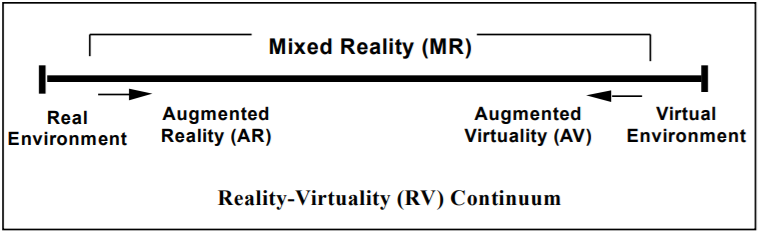
\includegraphics[width=0.95\textwidth]{Document/Figures/chapter1/RealityVirtualityContinuum.png}
    \caption[Simplified representation of a RV Continuum]{Simplified representation of a RV Continuum - from \cite{Milgram1994AugmentedContinuum}}
\end{figure}

To create the effect of AR a representation image of the real world and an overlaying digital image are required. Miligram et al. categorized AR display in two groups accordingly how the real world representation is put into practice. On one hand there are \textit{see-through AR displays} that brings the advantage of a direct contact to the actual surrounding - as this image is natural and not processed - and blend in object mostly with the help of mirror techniques. On the other hand there are \textit{monitor based AR displays} to which category the application using the Google Cardboard - resulting from this very project - can be counted to. In this representation modality the application gets and processes images coming from the reality as well as the digital counter part which are then fused and shown directly on one single display.

However those picture should not just be clashed together but be combined meaningfully in some way. That the effect of the reality being augmented can be created, the objects from the digital image has to integrate into the real world and have their specific place such as a real world object would have. This means, that it is important for the application to have somehow the knowledge of when to put which digital image into place, when the corresponding real world image is coming up. \cite{Kumar2017HowQuora} explains how the fusion can be done. There are two ideas that can be considered. 

One is the \textit{location-based} approach, where the application knows the position of a digital object that it would have in the real world. Assumed the application gets the precise data of the device - on which the AR is simulated - where its own location is, in what angle it is tilted and how much above the ground its lifted it would be possible to exactly calculate where and when the digital object should be overlaid. However the device does not see the real word as an image but instead has its representation based on those data provided. Testing my own device I noticed, that those data would not be very precise and therefore I will not really be able to use this approach for this project. More than that, the devices would need those data and would exclude every device and browser that does not provide them.

The other approach - that is that is also refereed as \textit{recognition-based Augmented reality} - is the \textit{marker-based} approach with the idea to tell the application when to show a certain object by giving hints in form of markers that are placed in the real world and therefore in the image send to the application. By analysing this pictures the application will recognize the marker and knows how to superimpose the corresponding digital parts. This approach will be used for this project.

Google Cardboard will serve to change a simple smartphone into a head-mounded device to create the possibility to immerse into this created AR. 
Basically Google Cardboard is just a box mostly made out of cardboard. Through a pair of lenses, serving as a magnifier, the viewer can see a split image in a way, such that each eye will just see its side of the picture. This enables a binocular vision which - when the pictures for each eye are different - results in a 3D effect. 
Any sort of a box in the style of the Google Cardboard should be usable for this project. However It might have to be adjusted a bit. As The real image will be taken directly by the camera of a device it is important to create a spare hole in the front of the box to provide the free view of the smartphone camera like like in figure \ref{fig:Google Cardboard b}.


\begin{figure}
	\begin{subfigure}[t]{0.45\textwidth}
		\centering
		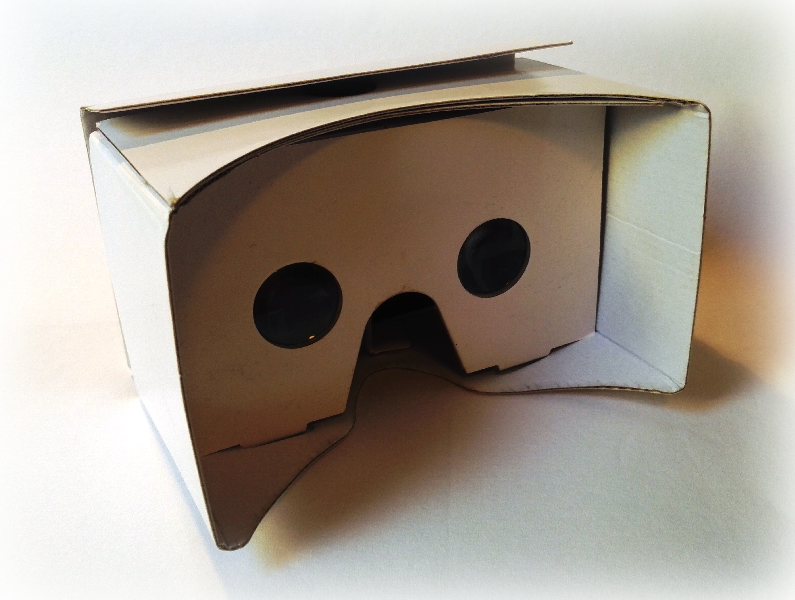
\includegraphics[height = 3.5cm]{Document/Figures/chapter1/GoogleCardboardRearView}
		\caption{}
		\label{fig:Google Cardboard a}
	\end{subfigure}
	\hfill
	\begin{subfigure}[t]{0.45\textwidth}
		\centering
		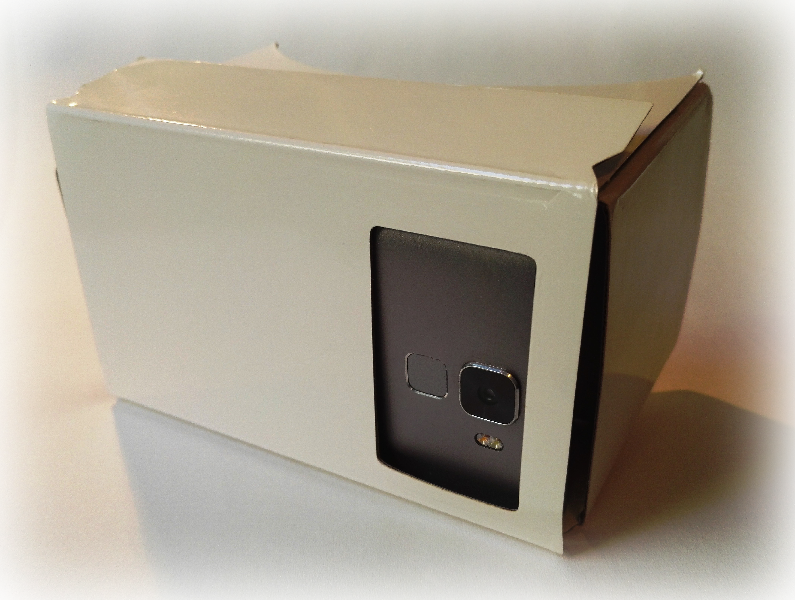
\includegraphics[height = 3.5cm]{Document/Figures/chapter1/GoogleCardboardFrontView}
		\caption{}
		\label{fig:Google Cardboard b}
	\end{subfigure}
	\caption[Google Cardboard with smartphone]
			{(a) Google Cardboard rear view where the two lenses are located.
			 (b) Google Cardboard front view with the spare hole for the smartphone camera.}
        \label{fig:Google Cardboard}
\end{figure}



For this project I was inspired by an article of \cite{Catanzariti2015AugmentedSitePoint}. Looking at the big tech companies producing products like the \textit{Meta Glasses}, \textit{Microsoft HoloLens} and \textit{Magic Leaphe} he pointed out, that those product were not quite accessible for an average consumer at that time and he thought of another way to put the concept into practice by creating a product for the mobile browser. This is a neat way to overcome the restriction of operating systems, however may be limited by the browser.

Catanzariti describes and showed by building his  \textit{AR LIFX Controller} \footnote{The \textit{AR LIFX Controller} can be found on GitHub at \url{https://github.com/sitepoint-editors/ARLIFXController}} how an AR application can be written with nothing more than some HTML and JavaScript files using the \textit{Awe.js} library that can be displayed on a mobile browser of a smartphone. He used the original code from this library which was created by \textit{buildAR.com} and is still accessible on GitHub\footnote{Original version of the old \textit{Awe.js} is available at \url{https://github.com/buildar/Awe.js}} however the code was declared as deprecated in 2016 and it was moved to a new GitHub repository. As mentioned and supposed by Catanzariti the team producing the library was quite active and published a new version - that also has a stereoscopic effect implemented - under the new producer name \textit{awe.media} on GitHub. This version got deprecated in 2017. After this point in time \textit{awe.media} moved their product to their own server and sells a service based on it on their web side \url{https://awe.media/}. 
They left their repository on GitHub and they even are keeping the deprecated version that can be freely accessed over the link \url{https://github.com/awe-media/Awe.js/tree/deprecated}. This is also the version that is used for this project to build on the AR Demo. For reference, the code of that version is also provided in the folder \textit{Applications} in the sub-directory \textit{Chapter1}. The repository is located in \textit{Source/third-party} as a ZIP-archive too. 

According the README.md\footnote{Online on GitHub at \url{https://github.com/awe-media/awe.js/blob/master/README.md}} on GitHub "the awe.js API sits on top of THREE.js and makes it easy for you to manage scenes, media objects, interactivity, sensors, device types and more."

However \textit{Awe.js} provides marker detection and the stereoscopic effect - beside some other features - those two functionalities are not yet combined in their version provided on GitHub. Assuming the yet hidden possibilities of that library - and combining those two features - it is used to approach the aim of this project that is to prove the possibility of creating an AR application on top of web technology - namely JavaScript and the necessary web APIs - combined with the Google Cardboard. The applications resulting form this work should be free and as easy as possible to access without special hardware, software or skills required in terms of consume or reproducing it.


\section{Method}

The final goal - the AR demo - will be approached in three steps:

\begin{enumerate}
\item  As \textit{Awe.js} sits on top of \textit{Three.js} this is the WebGL rendering library that will be setup, tested and evaluated to gain the basic knowledge of what is feasible and how \textit{Awe.js} possible could be tweaked. For every key point there will be an demo to see it in practice. The fist demo will be the very basic example of \textit{Three.js}. The other demo examples will build on top of this and be tweaked to achieve the desired result which is displaying and manipulating digital object in the browser. This step is described in chapter \ref{chp:WebGL Rendering Library}.

\item \textit{Awe.js} - as the actual AR library - will be setup, tested and evaluated. Again each key point will result in a small demo. Starting with one of the example - given in the \textit{Awe.js} ZIP-archive - adapted as base code. The knowledge from step could be helpful. A idea for the demo could be a digital chess figure standing on a real chessboard. This step is described in chapter \ref{chp:AR Library}.

\item Extending the final demo of step two with the stereoscopic effect and adapting it for the use of the Google Cardboard. This step is described in chapter \ref{chp:Google Cardboard AR demo}.

\end{enumerate}
After each step a small evaluation will be done.


I will develop on a \textit{Windows 10} machine, running \textit{Visual Studio Code} as editor. To view and inspect on the laptop the \textit{Google Chrome} browser will be used. To test on a mobile phone, I will use my \textit{Honor 7} with \textit{Android 6} and \textit{Google Chrome} mobile browser. As Google Cardboard I will use the one shown in figure \ref{fig:Google Cardboard}.

All created and used files will be place in the \textit{Applications} folder in a sub-directory accordingly to the chapter. A navigator - the \textit{index.html} file in the  \textit{Application} folder- will help getting an overview and access to the executable files and some references of the different application directly.


\section{Requirements}

For development I recommend to use \textit{Visual Studio Code} combined with the \textit{Live Server} extension by \cite{Dey2019LiveServer}.

To test and run, Chrome Browser will be preferred as it supports all feature that are used. Other combinations of OS and browser probably will fail. For more information read chapter TODO



 To be able to test all applications produced for this project, it is important to run them on a web server with https or when running on the local host that it is called with \textit{localhost:}.



Browser that supports \textit{WebGL} and TODO

gc to turn phone into a head mounted Device  


For development:


Setup web development environment

IDE from C9, belonging now to AWS (amazone web servises). Fortunatelly, any existing accounts still be working. New accounts have to registered in the new place (TODO). As an important point, it provides a server to run and test the code directly without having to setup any other applications than a browser e.g. Google Chrome. 


\begin{itemize}
\item 
\end{itemize}
any  code editor even plain text works
no os limitation

For final usage:
\begin{itemize}
\item Android phone with a Google Chrome as the mobile browser and a integrated camera
\item Google Cardboard with a spare hole for the phone camera
\item One or more printed markers 
\end{itemize}

server to run








-------------------------------------------------------






Each of those application must be developed for a certain operation system concerning the specific integration of hardware and software. 
The use of web technology, more concrete a web browser with the necessary API to use camera and some sort of GPU or even other useful features, could overcome the cap of the different operating systems. On one hand, it would ease the use and accessibility of such a web application, as no other application must be installed than a browser with the traits aforementioned. On the other hand, developing such an application would have the same nice restriction and advantages.





\section{Requirements}

For this project the following list is needed to achieve an AR application:
\begin{itemize}
    \item Server to run the code
    \item Engine to process and calculates the digital part
    \item Access to the smartphone camera and provider for the real environment imagery
    \item Display on which the results of the two aforementioned points are merge and shown.
\end{itemize}

For displaying and process, I rely on libraries which use JavaScript and WebGL. As alternative there would be Flash or 2dCanvas.

test for WebGL support visit https://get.webgl.org/



Requirements and technical evaluation
API for WebGl
API for Camera
Possible any API for other features like microphone
At a very basic level of understanding/abstraction, the device need to provide a camera for capturing a image of the real world and a browser in which the computation and display part will be executed. 
Chrome supports those desired feature (some table which show that) and provides a nice building debugging tool for JavaScript. For this reason, this project will mainly be tested and developed in chrome and as a smartphone, an android with the version 6.0. It will be possible, that specific problems could occur for the testing devices.









